\documentclass[journal, a4paper]{IEEEtran}
%\author{Huidong Lin}
% some very useful LaTeX packages include:

%\usepackage{cite}      % Written by Donald Arseneau
                        % V1.6 and later of IEEEtran pre-defines the format
                        % of the cite.sty package \cite{} output to follow
                        % that of IEEE. Loading the cite package will
                        % result in citation numbers being automatically
                        % sorted and properly "ranged". i.e.,
                        % [1], [9], [2], [7], [5], [6]
                        % (without using cite.sty)
                        % will become:
                        % [1], [2], [5]--[7], [9] (using cite.sty)
                        % cite.sty's \cite will automatically add leading
                        % space, if needed. Use cite.sty's noadjust option
                        % (cite.sty V3.8 and later) if you want to turn this
                        % off. cite.sty is already installed on most LaTeX
                        % systems. The latest version can be obtained at:
                        % http://www.ctan.org/tex-archive/macros/latex/contrib/supported/cite/

\usepackage{graphicx}   % Written by David Carlisle and Sebastian Rahtz
                        % Required if you want graphics, photos, etc.
                        % graphicx.sty is already installed on most LaTeX
                        % systems. The latest version and documentation can
                        % be obtained at:
                        % http://www.ctan.org/tex-archive/macros/latex/required/graphics/
                        % Another good source of documentation is "Using
                        % Imported Graphics in LaTeX2e" by Keith Reckdahl
                        % which can be found as esplatex.ps and epslatex.pdf
                        % at: http://www.ctan.org/tex-archive/info/

%\usepackage{psfrag}    % Written by Craig Barratt, Michael C. Grant,
                        % and David Carlisle
                        % This package allows you to substitute LaTeX
                        % commands for text in imported EPS graphic files.
                        % In this way, LaTeX symbols can be placed into
                        % graphics that have been generated by other
                        % applications. You must use latex->dvips->ps2pdf
                        % workflow (not direct pdf output from pdflatex) if
                        % you wish to use this capability because it works
                        % via some PostScript tricks. Alternatively, the
                        % graphics could be processed as separate files via
                        % psfrag and dvips, then converted to PDF for
                        % inclusion in the main file which uses pdflatex.
                        % Docs are in "The PSfrag System" by Michael C. Grant
                        % and David Carlisle. There is also some information
                        % about using psfrag in "Using Imported Graphics in
                        % LaTeX2e" by Keith Reckdahl which documents the
                        % graphicx package (see above). The psfrag package
                        % and documentation can be obtained at:
                        % http://www.ctan.org/tex-archive/macros/latex/contrib/supported/psfrag/

%\usepackage{subfigure} % Written by Steven Douglas Cochran
                        % This package makes it easy to put subfigures
                        % in your figures. i.e., "figure 1a and 1b"
                        % Docs are in "Using Imported Graphics in LaTeX2e"
                        % by Keith Reckdahl which also documents the graphicx
                        % package (see above). subfigure.sty is already
                        % installed on most LaTeX systems. The latest version
                        % and documentation can be obtained at:
                        % http://www.ctan.org/tex-archive/macros/latex/contrib/supported/subfigure/

\usepackage{url}        % Written by Donald Arseneau
                        % Provides better support for handling and breaking
                        % URLs. url.sty is already installed on most LaTeX
                        % systems. The latest version can be obtained at:
                        % http://www.ctan.org/tex-archive/macros/latex/contrib/other/misc/
                        % Read the url.sty source comments for usage information.

%\usepackage{stfloats}  % Written by Sigitas Tolusis
                        % Gives LaTeX2e the ability to do double column
                        % floats at the bottom of the page as well as the top.
                        % (e.g., "\begin{figure*}[!b]" is not normally
                        % possible in LaTeX2e). This is an invasive package
                        % which rewrites many portions of the LaTeX2e output
                        % routines. It may not work with other packages that
                        % modify the LaTeX2e output routine and/or with other
                        % versions of LaTeX. The latest version and
                        % documentation can be obtained at:
                        % http://www.ctan.org/tex-archive/macros/latex/contrib/supported/sttools/
                        % Documentation is contained in the stfloats.sty
                        % comments as well as in the presfull.pdf file.
                        % Do not use the stfloats baselinefloat ability as
                        % IEEE does not allow \baselineskip to stretch.
                        % Authors submitting work to the IEEE should note
                        % that IEEE rarely uses double column equations and
                        % that authors should try to avoid such use.
                        % Do not be tempted to use the cuted.sty or
                        % midfloat.sty package (by the same author) as IEEE
                        % does not format its papers in such ways.

\usepackage{amsmath}    % From the American Mathematical Society
                        % A popular package that provides many helpful commands
                        % for dealing with mathematics. Note that the AMSmath
                        % package sets \interdisplaylinepenalty to 10000 thus
                        % preventing page breaks from occurring within multiline
                        % equations. Use:
%\interdisplaylinepenalty=2500
                        % after loading amsmath to restore such page breaks
                        % as IEEEtran.cls normally does. amsmath.sty is already
                        % installed on most LaTeX systems. The latest version
                        % and documentation can be obtained at:
                        % http://www.ctan.org/tex-archive/macros/latex/required/amslatex/math/
\usepackage[outputdir=build]{minted}
\usepackage{amssymb}
\usepackage{amsmath}
\usepackage[hidelinks]{hyperref} 

\newcommand{\argmin}{\arg\!\min}
\newcommand{\argmax}{\arg\!\max}

% Other popular packages for formatting tables and equations include:

%\usepackage{array}
% Frank Mittelbach's and David Carlisle's array.sty which improves the
% LaTeX2e array and tabular environments to provide better appearances and
% additional user controls. array.sty is already installed on most systems.
% The latest version and documentation can be obtained at:
% http://www.ctan.org/tex-archive/macros/latex/required/tools/

% V1.6 of IEEEtran contains the IEEEeqnarray family of commands that can
% be used to generate multiline equations as well as matrices, tables, etc.

% Also of notable interest:
% Scott Pakin's eqparbox package for creating (automatically sized) equal
% width boxes. Available:
% http://www.ctan.org/tex-archive/macros/latex/contrib/supported/eqparbox/

% *** Do not adjust lengths that control margins, column widths, etc. ***
% *** Do not use packages that alter fonts (such as pslatex).         ***
% There should be no need to do such things with IEEEtran.cls V1.6 and later.


% Your document starts here!
\begin{document}
\begin{titlepage}

\newcommand{\HRule}{\rule{\linewidth}{0.5mm}} % Defines a new command for the horizontal lines, change thickness here

\center % Center everything on the page
 %----------------------------------------------------------------------------------------
%	LOGO SECTION
%----------------------------------------------------------------------------------------

~\\[1cm]
\includegraphics{/home/oidiotlin/Pictures/SCUT-full-logo.png}\\[2cm] % Include a department/university logo - this will require the graphicx package

%----------------------------------------------------------------------------------------
%	TITLE SECTION
%----------------------------------------------------------------------------------------

\HRule \\[1cm]
{ \huge \bfseries The Experiment Report of \textit{Machine Learning} }\\[0.6cm] % Title of your document
\HRule \\[2cm]
%----------------------------------------------------------------------------------------
%	HEADING SECTIONS
%----------------------------------------------------------------------------------------


\textsc{\LARGE \textbf{School:} School of Software Engineering}\\[1cm]
\textsc{\LARGE \textbf{Subject:} Software Engineering}\\[2cm] 

 
%----------------------------------------------------------------------------------------
%	AUTHOR SECTION
%----------------------------------------------------------------------------------------

\begin{minipage}{0.4\textwidth}
\begin{flushleft} \large
\emph{Author:}\\
Huidong Lin % Your name
\end{flushleft}
\end{minipage}
~
\begin{minipage}{0.4\textwidth}
\begin{flushright} \large
\emph{Supervisor:} \\
Qingyao Wu % Supervisor's Name
\end{flushright}
\end{minipage}\\[2cm]
~
\begin{minipage}{0.4\textwidth}
\begin{flushleft} \large
\emph{Student ID:}\\
201636665056
\end{flushleft}
\end{minipage}
~
\begin{minipage}{0.4\textwidth}
\begin{flushright} \large
\emph{Grade:} \\
Undergraduate
\end{flushright}
\end{minipage}\\[2cm]

% If you don't want a supervisor, uncomment the two lines below and remove the section above
%\Large \emph{Author:}\\
%John \textsc{Smith}\\[3cm] % Your name

%----------------------------------------------------------------------------------------
%	DATE SECTION
%----------------------------------------------------------------------------------------

{\large October 12, 2018}\\[2cm] % Date, change the \today to a set date if you want to be precise

 
%----------------------------------------------------------------------------------------

\vfill % Fill the rest of the page with whitespace

\end{titlepage}

% Define document title and author
	\title{Logistic Regression and Support Vector Machine}
	\maketitle

% Write abstract here
\begin{abstract}
% The short abstract is intended to give the reader an overview of the experiment. It should be brief and to the point. 
    This experiment intends to use logistic regression and linear classification respectively for binary classification problem, and update model parameters using mini-batch stochastic gradient descent.
\end{abstract}

% Each section begins with a \section{title} command
\section{Introduction}
	% \PARstart{}{} creates a tall first letter for this first paragraph
% \PARstart{T}{his} section introduces the problem to solved and leads the reader on to the main part. Detailed motivation is necessary. What's more, you can show your expected results and contributions.
    \PARstart{L}{ogistic} regression model and linear classification are used widely in machine learning field for binary classification problem. I reproduced these two algorithms with mini-batch SGD optimization methods and evaluated them on Adult Dataset of LIBSVM Data\footnote{LIBSVM Data - a9a: \url{https://www.csie.ntu.edu.tw/~cjlin/libsvmtools/datasets/binary.html\#a9a}}

% Main Part
\section{Methods and Theory}
% In this section, you are asked to give a complete introduction to the experiment. For instance, the chosen methods, the related theories, the related equations(loss function), the derivation process(taking the gradient) and so on.
\subsection{Logistic Regression}

\subsubsection{Model}

% Given a data set $\{y_i, x_i^{(1)}, \ldots, x_i^{(m)}\}_{i=1}^n$ of $n$ statistical units, a linear regression model assumes that the relationship between the dependent variable $y$ and the $m$-vector of regressors $\mathbf{x}$ is linear, which can be represented as

Assume a linear model:
    
\begin{equation}\label{eq:linear-model}
    \mathbf{z} = \boldsymbol\theta \cdot \mathbf{x}
\end{equation}        
    
Wrap it with an activation function call \textbf{sigmoid}:
    
\begin{equation}\label{eq:sigmoid}
    \sigma(x) = \frac{e^x}{e^x+1} = \frac{1}{1+e^{-x}}
\end{equation}
    
\begin{equation}\label{eq:logistic-h}
    h_{\boldsymbol\theta}(\mathbf{x}) = \sigma(\mathbf{z}) = \frac{1}{1+e^{-\boldsymbol\theta\cdot\mathbf{x}}}
\end{equation}

Apparently, $h_{\boldsymbol\theta}(\mathbf{x}) \in (0,1)$. Assume threshold is $\delta=0.5$.

\begin{equation}\label{eq:logistic-form}
    y = \left\{
    \begin{aligned}
        1 \qquad h_{\boldsymbol\theta}(\mathbf{x}) \geq \delta\\
        0 \qquad h_{\boldsymbol\theta}(\mathbf{x}) < \delta
    \end{aligned}
    \right.
\end{equation}

\subsubsection{Loss Function}

\eqref{eq:logistic-h} and \eqref{eq:logistic-form} can also be written in probability form:

\begin{equation}\label{eq:logistic-p}
    \begin{split}
        P(y = 1 | \mathbf{x};\boldsymbol\theta) & = h_{\boldsymbol\theta}(\mathbf{x}) \\
        P(y = 0 | \mathbf{x};\boldsymbol\theta) & = 1 - h_{\boldsymbol\theta}(\mathbf{x})
    \end{split}
\end{equation}

The likelihood function:

\begin{equation}\label{eq:likelihood}
    \begin{split}
        L(\boldsymbol\theta) & = \prod_{i=1}^{n} P(y_i|x_i;\boldsymbol\theta) \\
                             & = \prod_{i=1}^{n} (h_{\boldsymbol\theta}(x_i))^{y_i} \cdot (1-h_{\boldsymbol\theta}(x_i))^{1-y_i}
    \end{split}
\end{equation}

It is supposed to find the best $\boldsymbol\theta$:

\begin{equation}
    \boldsymbol{\theta}^{\ast} = \argmax_{\boldsymbol\theta}{L(\boldsymbol\theta)}
\end{equation}

Wrap $L(\boldsymbol\theta)$ with log function:

\begin{equation}\label{eq:log-likelihood}
    \begin{split}
        l(\boldsymbol\theta) & = \log(L(\boldsymbol\theta)) \\
                             & = \sum_{i=1}^{n}y_i \log \sigma(h_{\boldsymbol\theta}(x_i)) + (1-y_i)\log(1-\sigma(h_{\boldsymbol\theta}(x_i)))
    \end{split}
\end{equation}

For gradient descent, multiply it with $-\frac{1}{n}$:

\begin{equation}
    J(\boldsymbol\theta) = \frac{-1}{n}\sum_{i=1}^{n}y_i \log \sigma(h_{\boldsymbol\theta}(x_i)) + (1-y_i)\log(1-\sigma(h_{\boldsymbol\theta}(x_i)))
\end{equation}

Its gradient is:

\begin{equation}
    \begin{split}
        \nabla_{\boldsymbol\theta}J(\boldsymbol\theta) = & -y\cdot\frac{1}{h_{\boldsymbol\theta}(\mathbf{x})}\cdot\frac{\partial h_{\boldsymbol\theta}(\mathbf{x})}{\partial \boldsymbol\theta} \\
        & + (1-y)\cdot\frac{1}{1-h_{\boldsymbol\theta}(\mathbf{x})}\cdot\frac{\partial h_{\boldsymbol\theta}(\mathbf{x})}{\partial \boldsymbol\theta}
    \end{split}
\end{equation}

\subsection{Linear Classification}

\subsubsection{Model}

The linear model is the same as \eqref{eq:linear-model}.

\subsubsection{Loss Function}

Hinge-loss is used:

\begin{equation}
    H(\boldsymbol\theta) = \max(0, 1 - \mathbf{y}\dot h_{\boldsymbol\theta}(\textbf{x})
\end{equation}

Its gradient is:

\begin{equation}
    \nabla_{\boldsymbol\theta}H(\boldsymbol\theta) = - \textbf{x}\cdot\textbf{y}
\end{equation}

\section{Experiments}
\subsection{Dataset}
% This section represents the related information of datasets, such as the content, the number of data, the training set, the validation set and so on.

    There are 123 kinds of features in the dataset. The dataset has been divided into training and validation set with size $(32561, 16281)$ respectively. Each sample is labelled as $-1$ or $1$.

\subsection{Implementation}
\subsubsection{Initialization}
    Both of the two algorithm use random normal distribution for parameter $\boldsymbol\theta$ initialization.
    
    $$\boldsymbol\theta \sim N(\mu=1, \sigma^2=1)$$
    
\subsubsection{Parameters}
\paragraph{Logistic Regression}
    There are 4 hyper parameters in logistic regression as Table~\ref{tab:logistic-params} shown.
    \begin{table}[!hbt]
        \begin{center}
            \caption{Hyper Parameters of Logistic Regression}
            \label{tab:logistic-params}
            \begin{tabular}{l|l}
                \hline
                Parameters & Values \\
                \hline
                Number of epochs & $300$ \\
                Learning rate & $3\times 10^{-4}$ \\
                Batch size & $32$ \\
                $L2$-regularization factor & $0.4$ \\
                \hline
            \end{tabular}
        \end{center}
    \end{table}

\paragraph{Linear Classification}
    There are 4 hyper parameters in SGD algorithm as Table~\ref{tab:linear-params} shown.
    \begin{table}[!hbt]
        \begin{center}
            \caption{Hyper Parameters of Linear Classification}
            \label{tab:linear-params}
            \begin{tabular}{l|l}
                \hline
                Parameters & Values \\
                \hline
                Number of epochs & $250$ \\
                Learning rate & $8\times 10^{-3}$ \\
                Batch size & $512$ \\
                $L2$-regularization factor & $0.5$ \\
                \hline
            \end{tabular}
        \end{center}
    \end{table}
    
\subsubsection{Results}
\paragraph{Logistic Regression}
    Table~\ref{tab:logistic-losses} shows varying losses on different phases in the experiment. Figure~\ref{fig:logistic-losses} shows varying losses on training and validation set during training process.

    \begin{table}[!hbt]
        \begin{center}
        \caption{Log-likelihood Losses in Logistic Regression}
        \label{tab:logistic-losses}
        \begin{tabular}{l|l|l}
            \hline
            Phase & Dataset & Log-likelihood-Loss \\
            \hline
            Initialization & validation & $13.38$ \\
            Trained & training & $0.40$ \\
            Trained & validtion & $0.40$ \\
            \hline
        \end{tabular}
        \end{center}
    \end{table}   
     
    \begin{figure}[!hbt]
        \begin{center}
        \caption{Losses in Logistic Regression}
        \label{fig:logistic-losses}
        \includegraphics[width=\columnwidth]{../images/logistics-regression-losses.png}
        \end{center}
    \end{figure}
    
    \begin{figure}[!hbt]
        \begin{center}
        \caption{Accuracies in Logistic Regression}
        \label{fig:logistic-acc}
        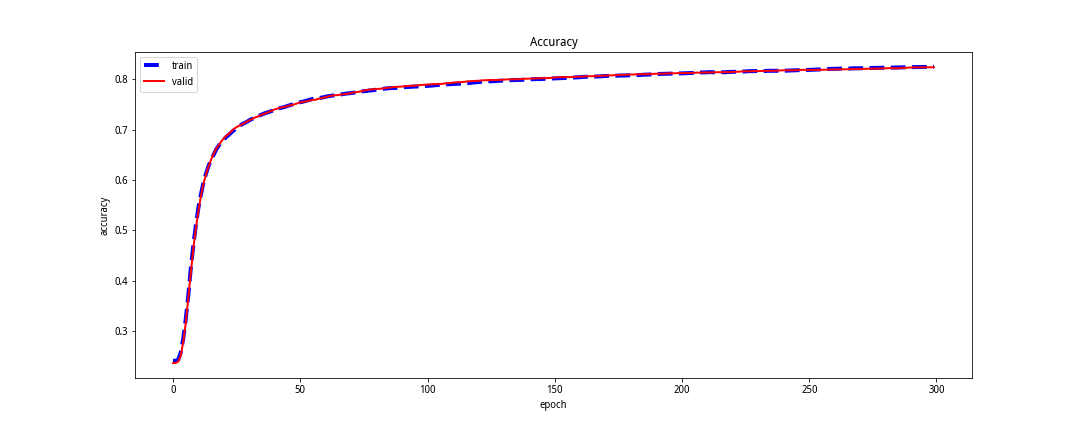
\includegraphics[width=\columnwidth]{../images/logistics-regression-accuracy.png}
        \end{center}
    \end{figure}

\paragraph{Linear Classification}
    Table~\ref{tab:linear-losses} shows varying losses on different phases in the experiment. Figure~\ref{fig:linear-losses} shows varying losses on training and validation set during training process.
    
    \begin{table}[!hbt]
        \begin{center}
        \caption{Hinge Losses in SGD}
        \label{tab:linear-losses}
        \begin{tabular}{l|l|l}
            \hline
            Phase & Dataset & Hinge-Loss \\
            \hline
            Initialization & training & $5.63$ \\
            Trained & training & $0.19$ \\
            Trained & validtion & $0.19$ \\
            \hline
        \end{tabular}
        \end{center}
    \end{table}
     
    \begin{figure}[!hbt]
        \begin{center}
        \caption{Losses in Linear Classification}
        \label{fig:linear-losses}
        \includegraphics[width=\columnwidth]{../images/linear-classification-losses.png}
        \end{center}
    \end{figure}
    
    \begin{figure}[!hbt]
        \begin{center}
        \caption{Accuracies in Linear Classification}
        \label{fig:linear-acc}
        \includegraphics[width=\columnwidth]{../images/linear-classification-accuracy.png}
        \end{center}
    \end{figure}

    
    The gradient descent is very smooth, which means that the descent process meets the requirements of this lab. In addition, the descent process of the loss of train and the loss of evaluation are similar, which means that the hyper-parameters chosen are suitable.

\section{Conclusion}
	This experiment is much more interesting than the first experiment. With slides provided by Mr. Wu, it is much easier to calculate the derivation of these two loss function.


% Your document ends here!
\end{document}